% ------------------------------------------------------------------------------
% Revisão Bibliográfica
% ------------------------------------------------------------------------------

\chapter{Revisão Bibliográfica}\label{chap:revisao}

\section{Ciclo de Vida}\label{sec:revisao:ciclodevida}

	A definição e criação de um ciclo de vida é uma das formas de a Engenharia de Sistemas (ES) atuar em seu propósito de viabilizar o sucesso de um sistema, ao mesmo tempo em que otimiza a concorrência existente entre os objetivos das partes interessadas. Ao desmembrar o esforço total e definir os estágios, seus papéis, as novas características do sistema, os critérios de conclusão, os riscos envolvidos e, finalmente, tomar uma decisão, está-se criando o ciclo de vida. Esse processo organiza e estrutura as etapas necessárias para o desenvolvimento e a evolução do sistema de forma clara e eficiente.

	Entre cada estágio definido, existem os chamados \textit{decision gates} (portões de decisão, em tradução livre). Nesses pontos, realiza-se uma análise do progresso e, como o nome sugere, toma-se uma decisão em relação ao desenvolvimento do sistema.

	O ciclo de vida de um sistema é definido a partir de suas características e particularidades, de modo que seus estágios sejam inseridos para atender a todas as suas necessidades. Os estágios podem ocorrer mais de uma vez, ser executados sequencialmente ou paralelamente, e ser inseridos em qualquer momento do ciclo de vida.

	Em alguns casos, o Sistema de Interesse (SoI, do inglês \textit{System of Interest}) faz parte de um Sistema de Sistemas (SoS, do inglês \textit{System of Systems}). Nesse contexto, cada um possui seu próprio ciclo de vida. Geralmente, em um SoS, cada elemento do sistema tem um ciclo de vida independente, e o ciclo de vida do SoS influencia diretamente o do SoI. Por isso, ao analisar o ciclo de vida do SoI, é essencial considerar sua evolução e as interações com o SoS.

	O ciclo de vida genérico apresentado em \cite{incoseHandbook} mostra os seis estágios básicos organizados em uma estrutura em ``V'', que busca representar visualmente a ocorrência desses estágios ao longo do tempo, destacando também o possível paralelismo entre eles. Os estágios são: conceito, desenvolvimento, produção, utilização, suporte e descontinuação. A Figura~\ref{fig:revisao:veeLifeCycle} ilustra essa representação conforme apresentada no livro. A seguir, cada estágio será abordado:

	\begin{figure}[h]
		\centering
		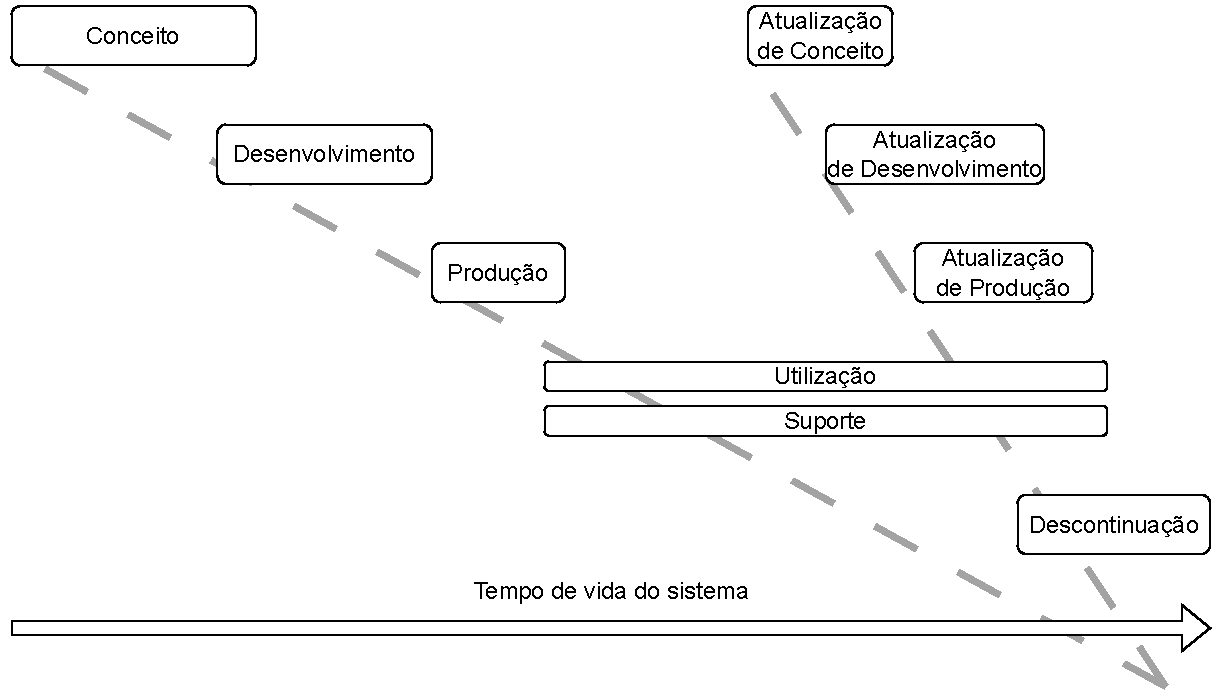
\includegraphics[width=\textwidth]{./figuras/veeLifeCycle.pdf}
		\caption{Ciclo de vida com estrutura em ``V''.}
		\label{fig:revisao:veeLifeCycle}
	\end{figure}

	\begin{itemize}
		\item \textbf{Estágio de conceito}: Este estágio representa a fase exploratória, em que são identificadas as origens de uma necessidade, uma nova missão, uma nova capacidade de negócio ou a modificação de algum desses elementos. Nele, são analisados diversos fatores do sistema, como o mercado, aspectos ambientais, condições econômicas, recursos disponíveis e o escopo de atuação. O objetivo é definir os limites do problema a ser resolvido, as missões do sistema, onde ele será aplicado, além de realizar uma análise do negócio, da missão e dos valores a serem entregues. Para garantir uma definição clara do problema, são realizados levantamentos dos requisitos do sistema, das partes interessadas envolvidas e de suas necessidades, além da exploração do espaço de soluções possíveis. Com base nisso, é possível estimar um custo inicial do esforço necessário e criar uma agenda preliminar, que servirá como base para o ciclo de vida do sistema. Alguns dos resultados típicos desse estágio incluem documentos preliminares de arquitetura do sistema, análise de viabilidade, requisitos, design, cronograma e estimativa de esforço. Esse estágio é crucial, pois é nele que o sistema é definido. Embora mudanças possam ocorrer posteriormente, sua implementação tende a ser mais complexa e custosa devido a fatores como tempo e recursos adicionais.

		\item \textbf{Estágio de desenvolvimento}: Nesse estágio, é definido um SoI que atende às necessidades e aos requisitos das partes interessadas, e que pode ser produzido, utilizado, suportado e descontinuado, se necessário. O objetivo principal dessa fase é definir um projeto-base de engenharia que possa ser executado, sem buscar a perfeição, mas atendendo às partes interessadas e respeitando os possíveis \textit{trade-offs} previamente identificados. Esse projeto-base deve conter os requisitos, a arquitetura, modelagens, documentação e o planejamento para as próximas fases — todos considerados também como produtos dessa etapa.

		\item \textbf{Estágio de produção}: Nesse estágio, o projeto-base definido no desenvolvimento é aprovado e qualificado para ser implementado. Representa o momento de transição para um ambiente produtivo real, incluindo a instalação, montagem, fabricação e testes de aceitação.

		\item \textbf{Estágio de utilização}: O início deste estágio ocorre com a liberação do sistema — ou de partes dele — para uso, incluindo os sistemas de apoio necessários para certas funcionalidades. Este é, comumente, o estágio mais longo do ciclo de vida. Alterações e melhorias no SoI costumam surgir ao longo do tempo, exigindo atenção contínua ao gerenciamento de riscos e à documentação, a fim de garantir a integridade e a manutenção do sistema.

		\item \textbf{Estágio de suporte}: Este estágio ocorre em paralelo ao de utilização, a partir do momento em que alguma funcionalidade se torna disponível. No entanto, seu planejamento e preparação podem começar antes, com ações como a aquisição de sobressalentes. É durante essa fase que se percebem oportunidades de melhorias e mudanças a serem implementadas durante a operação do sistema.

		\item \textbf{Estágio de descontinuação}: Esse estágio ocorre quando o sistema é oficialmente retirado de operação, marcando o encerramento dos estágios de utilização e suporte, podendo haver pequena sobreposição entre eles. Além de definir como será realizado o descarte ou o armazenamento físico ou digital dos componentes do sistema, essa etapa também envolve a análise da possível extensão da vida útil de certos elementos e o arquivamento dos documentos importantes relacionados. Trata-se de uma fase essencial para garantir o encerramento adequado do ciclo de vida do sistema.
	\end{itemize}

	
	Ainda no \cite{incoseHandbook}, são apresentados conceitos importantes sobre os \textit{decision gates}, que coexistem entre os estágios do ciclo de vida, tanto no início quanto no fim de cada etapa. 

	Entre os objetivos dos \textit{decision gates}, destacam-se: o acompanhamento da evolução da maturidade do sistema, a verificação dos critérios de entrada e saída de cada estágio, a análise de riscos com base na situação atual do sistema e, por fim, a tomada de decisão quanto ao próximo passo. Essa decisão pode resultar no avanço para o estágio seguinte, no retorno a um estágio anterior, na interrupção temporária ou até mesmo no cancelamento do projeto.

	É fundamental equilibrar o nível de formalidade e a frequência desses eventos, uma vez que envolvem diversas partes interessadas, gestores e especialistas. Além disso, as decisões devem ser fundamentadas em dados coletados nos estágios do ciclo de vida e nos artefatos produzidos para esse fim. Isso evita decisões desnecessárias ou inadequadas que possam comprometer o projeto no futuro.

	O \cite{incoseHandbook} também apresenta três abordagens principais para a modelagem dos ciclos de vida: sequencial, incremental e evolucionária. As principais características dessas três abordagens estão resumidas na Tabela~\ref{tab:revisao:ciclodevida:abordagens}.

	\begin{table}[!h]
		\centering
		\caption{Características das abordagens de um ciclo de vida}
		\begin{tabular}{cccc}
			\hline
			Abordagem & Requisitos definidos no ínicio & Iterações planejadas & Múltiplas instalações \\
			\hline
			Sequencial & Todos os requisitos & Apenas uma & Não\\
			Incremental & Todos os requisitos & Múltiplas & Potencialemnte\\
			Evolucionário & Parte dos requisitos & Múltiplas & Tipicamente\\
			\hline
		\end{tabular}
		\label{tab:revisao:ciclodevida:abordagens}
	\end{table}

	Durante a execução dos estágios do ciclo de vida, várias tarefas são executadas, e, para isso, alguns processos precisam ser realizados para garantir a consistência das atividades. Um conjunto de processos é definido no livro, e a execução de cada um deles varia de acordo com os estágios existentes no ciclo de vida do sistema.

	\subsection{Fases dos estágios de Conceito e Desenvolvimento}\label{sec:revisao:ciclodevida:fases}

	\cite{kossiakoff2020systems} fazem uma quebra dos estágios de conceito e desenvolvimento citados anteriormente, subdividindo-os em três fases cada. Dessa maneira, a análise do ciclo de vida
	de um sistema, bem como a sua estruturação, fica mais clara e objetiva.
	Para o estágio de conceito, temos as fases mostradas na Figura~\ref{fig:revisao:conceptStagePhases}; \cite{kossiakoff2020systems} as descreve da seguinte maneira:

	\begin{figure}[h]
		\centering
		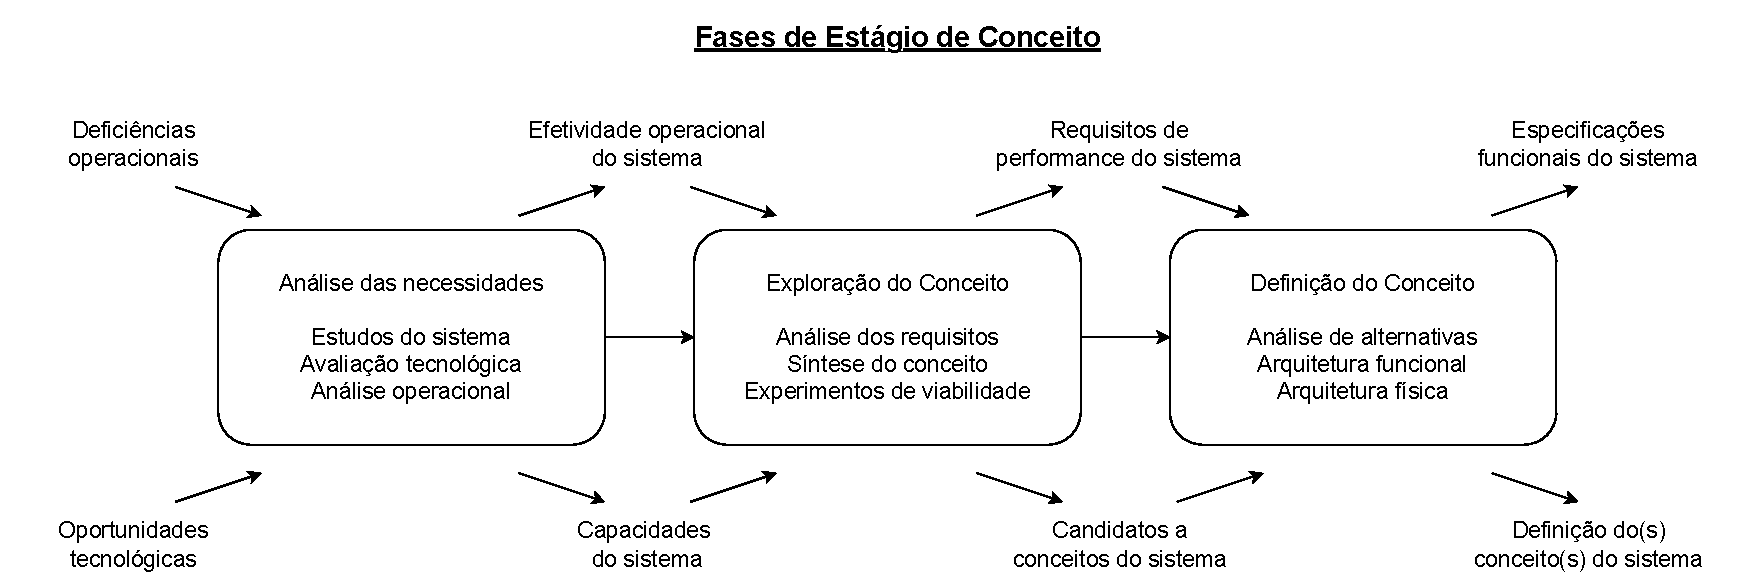
\includegraphics[width=\textwidth]{./figuras/conceptPhases.pdf}
		\caption{Fases do estágio de Conceito, adaptado de \citep{kossiakoff2020systems}}
		\label{fig:revisao:conceptStagePhases}
	\end{figure}

	\subsubsection*{Fase de análise de necessidade}

	A fase de análise de necessidades tem como objetivo identificar se há, de fato, uma necessidade legítima para o desenvolvimento de um novo sistema, bem como 
	avaliar se existe uma abordagem viável para atendê-la. Essa etapa exige uma análise crítica das limitações dos meios existentes em
	suprir as demandas atuais ou futuras previstas. Também é considerada a viabilidade técnica, ou seja, se a tecnologia disponível é capaz de suportar a 
	capacidade adicional desejada.

	Frequentemente, o início do ciclo de vida de um sistema não se dá de forma repentina, mas sim como resultado de uma análise contínua das necessidades 
	operacionais ou do desenvolvimento de produtos inovadores. O principal resultado dessa fase é a descrição das capacidades e da efetividade operacional 
	esperadas do novo sistema. Embora ainda não configure um conjunto formal de requisitos, essa 
	descrição serve como base para sua futura definição.

	Para apoiar essa fase, são utilizados diversos métodos e ferramentas, especialmente das áreas da análise operacional e da pesquisa operacional. Além disso, 
	avaliações tecnológicas e experimentações complementam essas abordagens matemáticas, contribuindo para uma definição mais precisa das necessidades do sistema.

	\subsubsection*{Fase de exploração de conceito}

	Na fase de exploração de conceitos, busca-se responder às seguintes questões: ``Qual desempenho o novo sistema precisa atingir para satisfazer a necessidade 
	identificada?'' e ``Existe pelo menos uma abordagem viável para alcançar esse desempenho a um custo aceitável?'' A resposta positiva a essas perguntas é essencial 
	para estabelecer objetivos realistas e viáveis antes de investir fortemente no desenvolvimento do sistema.

	O principal resultado desta fase é a formulação do primeiro conjunto de requisitos de desempenho do sistema, considerados ``oficiais'' por serem passíveis de 
	medição e avaliação por parte de contratantes ou agências. Além disso, são gerados os conceitos candidatos de sistema — ou seja, múltiplas alternativas de 
	solução. A exploração de diferentes abordagens é fundamental para compreender as possibilidades disponíveis para atender à necessidade identificada.

	Diversas ferramentas e técnicas são utilizadas nessa etapa, incluindo métodos de processo (como análise de requisitos) e julgamento especializado 
	(como sessões de brainstorming). Inicialmente, o número de conceitos pode ser elevado, mas o processo visa reduzi-los 
	rapidamente a um conjunto manejável. A viabilidade das alternativas finais precisa ser comprovada, pois elas serão a base para as decisões da próxima fase do 
	ciclo de vida.

	\subsubsection*{Fase de definição de conceito}

	A fase de definição de conceito tem como foco selecionar o conceito de sistema mais promissor, ou seja, aquele que apresenta o melhor equilíbrio entre 
	capacidade, vida útil operacional e custo. Para isso, diferentes alternativas devem ser comparadas em relação ao desempenho, utilidade operacional, riscos 
	de desenvolvimento e custos. Com base nessa análise, é decidido se vale a pena investir recursos significativos no desenvolvimento do novo sistema.

	O principal resultado dessa fase é uma descrição funcional clara do que o sistema deve fazer e qual desempenho deve alcançar, além da definição do conceito 
	selecionado de sistema. Em sistemas simples, essa descrição pode ser feita de forma direta; em sistemas mais complexos, é necessária uma arquitetura de sistema 
	mais detalhada, que represente o sistema sob diferentes perspectivas — principalmente funcional e física.

	As ferramentas utilizadas nesse estágio incluem análise de alternativas e práticas de arquitetura de sistemas. Em contextos comerciais, as 
	fases anteriores são frequentemente integradas em um estudo de viabilidade, que serve como base para decidir se o conceito deve ser desenvolvido.

	Mesmo que já tenham sido dedicados esforços significativos na compreensão do ambiente operacional e das tecnologias relacionadas, até este ponto o 
	investimento direto no desenvolvimento do sistema costuma ser limitado. É nas fases seguintes que a maior parte dos recursos será aplicada, com foco no 
	desenvolvimento técnico e implementação.

	Olhando agora para o estágio de desenvolvimento, vemos na Figura~\ref{fig:revisao:developmentStagePhases} suas fases, bem como entradas e saídas. Novamente, suas definições, segundo \cite{kossiakoff2020systems}, encontram-se abaixo:

	\begin{figure}[h]
		\centering
		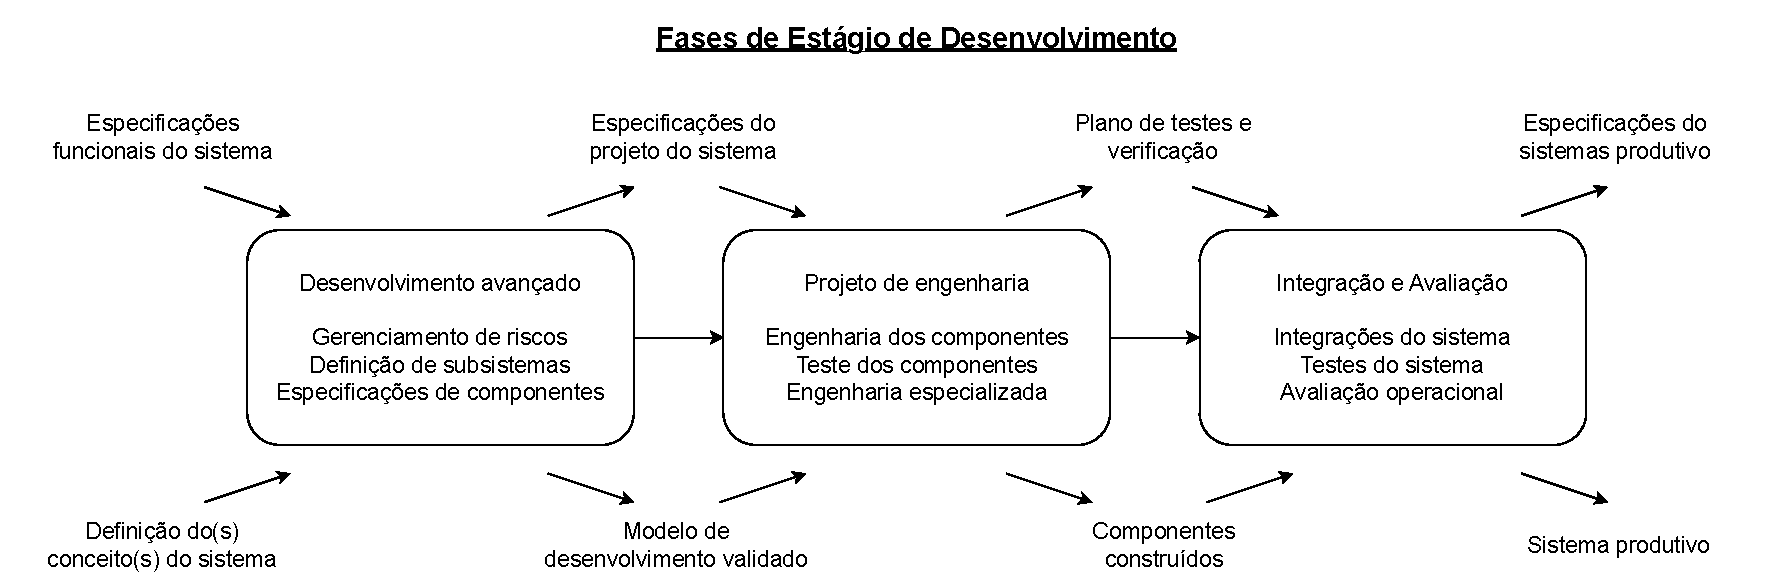
\includegraphics[width=\textwidth]{./figuras/developmentPhases.pdf}
		\caption{Fases do estágio de Desenvolvimento, adaptado de \citep{kossiakoff2020systems}}
		\label{fig:revisao:developmentStagePhases}
	\end{figure}


	\subsubsection*{Fase de desenvolvimento avançado}
	A fase de desenvolvimento avançado marca a transição entre a definição conceitual e o início do desenvolvimento técnico de um sistema. Seu sucesso depende 
	fortemente da solidez das decisões tomadas nas fases conceituais anteriores. No entanto, como essas fases iniciais geralmente envolvem análises com recursos 
	limitados, ainda restam incertezas importantes que precisam ser identificadas e resolvidas o quanto antes. Esta fase tem como principal objetivo minimizar 
	esses riscos e transformar os requisitos funcionais do sistema em especificações técnicas mais detalhadas.

	Duas finalidades centrais definem esta fase: a identificação e mitigação de riscos de desenvolvimento e a produção das especificações de design do sistema. 
	Isso é particularmente crítico em projetos que envolvem tecnologias inovadoras ou desempenho que extrapola os limites previamente testados. A fase 
	concentra-se no desenvolvimento e validação das partes do sistema que ainda não estão consolidadas, assegurando que seus requisitos possam, de fato, ser 
	atendidos.

	Nesta etapa, a ES desempenha papel essencial ao definir o que precisa ser validado, como isso será feito e como interpretar os resultados 
	obtidos. Frequentemente, modelos experimentais e simulações são empregados para validar conceitos de projeto de componentes e subsistemas, reduzindo os custos 
	de desenvolvimento.

	O produto final desta fase é um modelo de desenvolvimento validado, junto a um conjunto refinado de especificações de projeto. Esse modelo deve demonstrar que
	o sistema pode ser projetado e fabricado de forma viável e com riscos aceitáveis. Por isso, todos os riscos precisam estar classificados como controláveis 
	antes que o projeto avance para a próxima fase do ciclo de vida.

	\subsubsection*{Fase de projeto de engenharia}

	A fase de projeto de engenharia representa a transição entre a definição conceitual e a concretização técnica do sistema. É nesta etapa que o projeto detalhado 
	dos componentes é desenvolvido, resultando na criação de um protótipo funcional ou virtual do sistema. Devido à sua complexidade e escopo, essa fase é geralmente
	marcada por revisões formais de projeto, que permitem ao cliente acompanhar o progresso, controlar custos, revisar o cronograma e fornecer feedback essencial 
	aos desenvolvedores.

	Embora aspectos como confiabilidade, manutenibilidade e fabricabilidade – conhecidos como ``Engenharia especializada'' – já tenham sido considerados anteriormente, 
	nesta fase eles assumem um papel central. O engenheiro de sistemas tem a responsabilidade de garantir que cada componente implementa corretamente os requisitos 
	funcionais e de compatibilidade, além de coordenar o processo de mudanças de engenharia para manter o controle das interfaces e da configuração do sistema.

	As principais atividades dessa etapa incluem a conversão das especificações de componentes em projetos de engenharia completos, além da execução de testes 
	preliminares. Esses testes podem ser realizados imediatamente após o projeto ou paralelamente a ele. Outro elemento crucial é o refinamento do plano de testes e 
	avaliações (T\&A), iniciado em fases anteriores, mas consolidado com base nas decisões e dados acumulados até aqui.

	Os dois principais produtos desta fase são o plano de T\&A e um protótipo do sistema. Este protótipo pode assumir diferentes formas — física, virtual ou híbrida — 
	dependendo da natureza do sistema em questão. Por exemplo, no caso de sistemas complexos e de grande escala, como embarcações de carga, o protótipo pode combinar
	simulações digitais e modelos físicos em escala reduzida.

	Ferramentas modernas de projeto assistido por computador (CAD) e simulações de sistemas são amplamente utilizadas para apoiar as decisões de engenharia, 
	garantindo que o sistema projetado seja viável, testável e alinhado com os objetivos operacionais definidos nas fases iniciais do ciclo de vida.

	\subsubsection*{Fase de integração e avaliação}
	A fase de integração e avaliação marca o momento em que os componentes projetados e desenvolvidos são reunidos para formar um sistema funcional completo. 
	Embora ainda seja parte do processo de desenvolvimento, essa etapa possui características distintas, especialmente no que diz respeito ao papel da ES, 
	justificando seu tratamento como uma fase separada no ciclo de vida do sistema.

	É nessa etapa que o sistema é montado e testado pela primeira vez em um ambiente realista ou simulado. Isso permite verificar se as interfaces entre os 
	componentes estão compatíveis e se a integração geral atende aos requisitos funcionais estabelecidos. Apesar de testes prévios em subsistemas ou protótipos 
	terem sido realizados, somente agora é possível validar a integridade do sistema como um todo.

	Frequentemente, a execução dessa fase exige a construção de instalações específicas capazes de simular estímulos operacionais e restrições reais, de modo a 
	permitir uma avaliação precisa do desempenho do sistema. A complexidade e os recursos necessários para essa infraestrutura não devem ser subestimados.

	Os principais resultados da fase de integração e avaliação são: (i) as especificações finais de produção do sistema, conhecidas como ``baseline de produção'', 
	que orientam a fabricação do produto final, e (ii) o sistema de produção propriamente dito, que inclui tudo o que é necessário para manufaturar e montar o 
	sistema em escala.

	Ferramentas modernas de integração, T\&A, bem como métodos e princípios atualizados, estão disponíveis para apoiar os engenheiros nesse processo. Antes que a 
	produção em larga escala possa começar, é essencial que o sistema final seja verificado e validado em um ambiente operacional real ou em uma simulação que represente 
	fielmente esse contexto.

	
	\cite{kossiakoff2020systems} trazem ainda um relacionamento entre as fases desses dois estágios com os níveis de detalhamento do sistema. De maneira visual, é destacado
	em quais níveis cada fase deve alcançar, consequentemente definindo o detalhamento de cada fase. Assim, fica mais clara a materialização do sistema, onde as primeiras fases tocam
	na parte mais superficial e mais abstrata, e, à medida que se avança de fase, vai-se adentrando nos níveis de funcionalidades, quebrando e detalhando as funções e associando-as com
	os elementos do sistema no nível correspondente. A tabela \ref{tab:revisao:systemMaterialization} ilustra essas relações.

	É fundamental perceber que, mesmo que o projeto detalhado só se conclua tardiamente no
	desenvolvimento, a visualização geral do sistema deve ocorrer ainda nas fases iniciais.
	Isso é necessário para estimar custos, viabilidade técnica e orientar a escolha do conceito do sistema.
	A visualização inicial não precisa ser precisa em todos os detalhes, mas deve ser realista o suficiente
	para orientar decisões viáveis.

	\begin{table}[H]
		\centering
		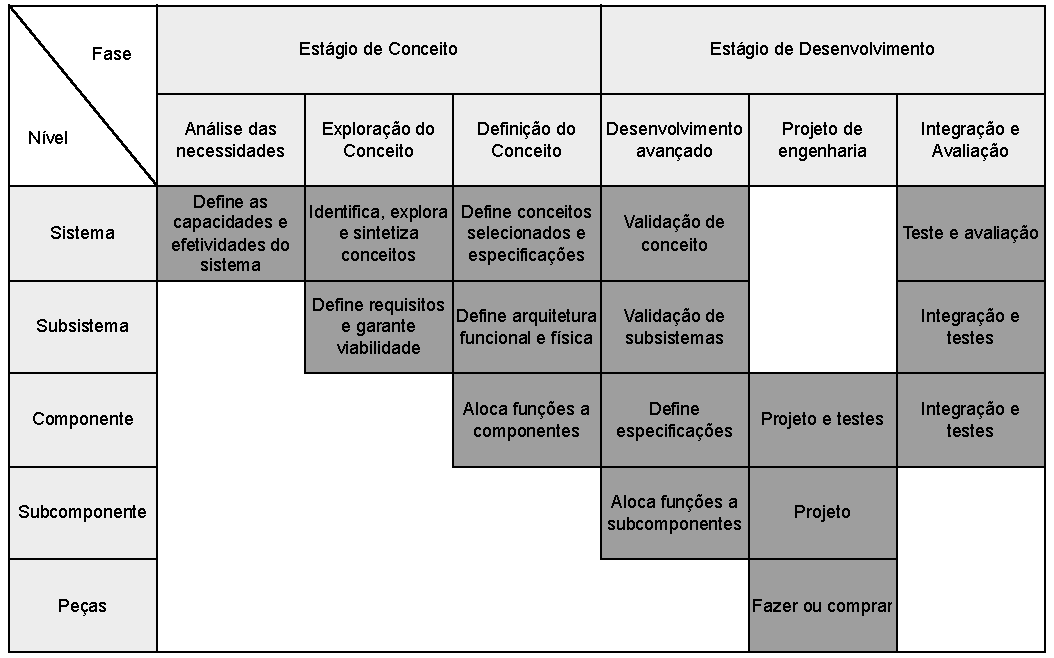
\includegraphics[width=\textwidth]{./figuras/systemMaterialization.pdf}
		\caption{Materialização do sistema, adaptado de \citep{kossiakoff2020systems}}
		\label{tab:revisao:systemMaterialization}
	\end{table}

	\subsection{Estágios de Pós Desenvolvimento}\label{sec:revisao:ciclodevida:posDev}
	Após a conclusão do desenvolvimento de um sistema, inicia-se a etapa pós-desenvolvimento, composta por duas fases principais, de acordo com
	\citep{kossiakoff2020systems}: Produção e Utilização e Suporte. Os autores unificaram Utilização e Suporte, pois, de fato, seguem em paralelo a todo momento.
	Porém, será adicionado o último estágio do ciclo de vida apresentado pelo \cite{incoseHandbook} a esse grupo, o estágio de Descontinuação. A figura
	\ref{fig:revisao:postDevelopment} traz, no mesmo estilo, a representação desses estágios.

	\begin{figure}[h]
		\centering
		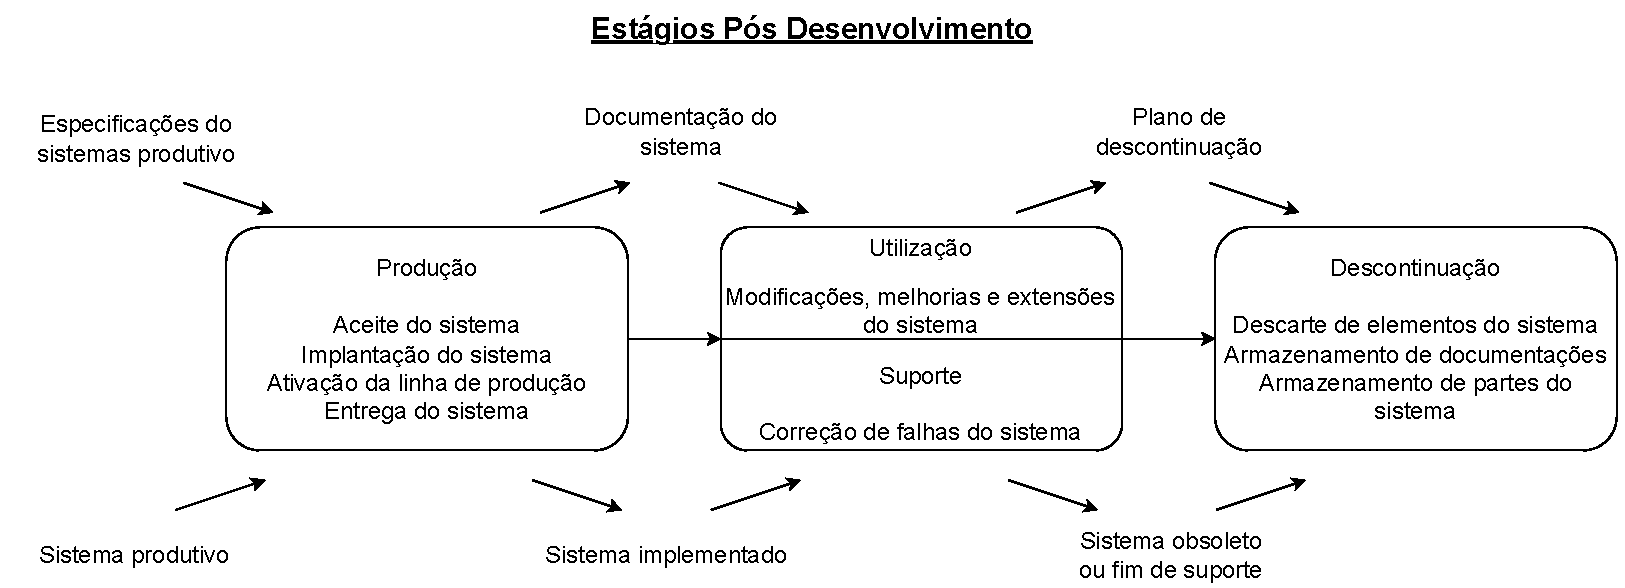
\includegraphics[width=\textwidth]{./figuras/postDevelopment.pdf}
		\caption{Estágio de Pós Desenvolvimento, adaptado de \citep{kossiakoff2020systems}}
		\label{fig:revisao:postDevelopment}
	\end{figure}
	
	\section{Arquitetura do Sistema}\label{sec:revisao:arqSistema}

	Como mencionado na seção \ref{sec:revisao:ciclodevida}, existem diferentes etapas durante o ciclo de vida de
	um sistema. Uma delas é o ``Processo de Definição da Arquitetura do Sistema'', que tem como objetivo, conforme registrado
	no \cite{incoseHandbook}, gerar alternativas de arquiteturas do sistema, selecionar uma ou mais alternativas que atendam aos
	requisitos das partes interessadas, e expressar isso em uma visualização e modelos consistentes.

	Dessa forma, esse processo provê informação e dados necessários para identificar e caracterizar os conceitos e
	propriedades fundamentais do sistema e seus elementos. Esse processo é vivo ao longo do ciclo de vida, e deve ser sempre
	retomado quando há modificações de conceitos ou de perspectivas no decorrer do desenvolvimento do sistema.

	Dentre as entradas para a execução desse processo mostradas no \cite{incoseHandbook}, destacam-se os ``Requisitos do Sistema'',
	as ``Restrições de solução'', a ``Descrição do projeto do sistema'', ``As soluções alternativas'' e um ``Projeto de arquitetura validado e verificado''.

	Com essas entradas em mãos são realizadas as atividades para a definição de qual será a arquitetura definitiva do sistema. E, após
	isso, temos como saídas resultantes típicas os ``Artefatos e registros da arquitetura do sistema definida'', a ``Descrição da 
	arquitetura do sistema'', o ``Mapeamento de rastreabilidade'' e a ``Justificativa da arquitetura do sistema''.
	 
	A existência de um ``Estilo de Arquitetura'' é de extrema importância para que esse processo seja executado com êxito.
	Ele atua como um modelo, ou guia, para se construir a arquitetura do sistema. Os ``Estilos de Arquitetura'' podem 
	ser definidos com base nos pontos de vista da arquitetura, nos elementos do
	sistema e seus relacionamentos, nas conexões, interfaces, mecanismos de interação e possíveis restrições.
	
	Além dos ``Estilos de Arquitetura'', outro conceito importante é o de ``Padrões de Arquitetura''. 
	Eles são modelos simplificados, mas completos no que diz respeito aos elementos do
	sistema e são reutilizáveis para diferentes tipos de cenários. O uso de ``Padrões de Arquitetura'' agiliza a 
	documentação, facilita a comunicação, promove o reúso, melhora a produtividade
	e eficiência e serve como um ponto de início para o desenvolvimento de novos sistemas.

	Como o conceito de arquitetura pode ser muito abrangente, o \cite{sebok2024} mostra três segmentações: a arquitetura funcional, lógica e a física.

	A arquitetura funcional compreende as funcionalidades do sistema, ou seja, quais funções ou comportamentos 
	aquele sistema executa ou possui em diferentes contextos para atingir os objetivos esperados pelos diferentes interessados.
	Essa arquitetura está fortemente conectada com a definição de conceito do sistema e tem papel chave em dar início à materialização do sistema,
	ao traduzir esses conceitos em um projeto de sistema viável. Não há exatamente um modelo ou padrão recomendado de
	arquitetura funcional; em casos de sistemas com poucas funcionalidades ou menos complexos, um texto descritivo já seria 
	suficiente; em outros casos, um diagrama hierárquico de funcionalidades pode ser mais interessante. Essa arquitetura é 
	construída já no primeiro estágio do ciclo de vida do sistema.

	O desenvolvimento da arquitetura lógica tem como propósito definir, sintetizar e documentar a lógica por trás do sistema a ser desenvolvido,
	resultando em uma modelagem que poderá ser utilizada, no futuro, para verificar e validar os requisitos do sistema em todos os cenários operacionais.
	Essa arquitetura pode incluir mais de um artefato, como um modelo de arquitetura funcional decomposta em hierarquia de funções e subfunções, um modelo de arquitetura comportamental com diagramas
	de atividades, de estados, de fluxos de dados ou de blocos funcionais do sistema, e ainda um modelo de arquitetura temporal do sistema, com as funções do sistema 
	classificadas de acordo com a frequência de execução, podendo incluir também os aspectos síncronos e assíncronos do sistema.

	Já na definição da arquitetura física há o propósito de elaborar modelos e visualizações concretas de soluções que acomodem a arquitetura
	lógica e que atendam aos requisitos do sistema conforme acordado. A arquitetura física é uma organização dos elementos do sistema
	que compõem a solução, seja ela um produto, um serviço ou até mesmo uma empresa. Como existem diferentes tipos de sistema, o elemento do sistema pode
	assumir diferentes características ou interfaces; em produtos, eles podem ser de fato componentes físicos mecânicos ou eletrônicos, podem ser softwares
	específicos e papéis de operação; já para serviços, por exemplo, eles podem ser bancos de dados, processos, papéis de operação, aplicações.
	Nesse momento é feita a associação dos elementos lógicos do sistema, derivados dos requisitos, aos elementos físicos do sistema, gerando então o mapeamento de rastreabilidade.
	Mais de uma abordagem de arquitetura pode ser sugerida às partes interessadas, que devem analisar e escolher a que melhor atende. Essa modelagem pode ser feita utilizando
	diagramas de estrutura de blocos e layouts ou outros modelos que podem variar de acordo com o domínio em que o sistema está envolvido.

	\section{Trabalhos relacionados}

	\subsection{Low Code Development Cycle Investigation}

	O uso de \textit{low code} nas organizações tem diferentes motivos. Um deles é o empoderamento de seus funcionários, como citado por \cite{LowCodeLifeCicle}.
	Ao qualificar e incentivar os funcionários a utilizarem essas tecnologias para resolverem seus problemas, são criadas comunidades de \textit{citizen developers}, que, em tradução livre, podem ser
	chamados de ``desenvolvedores cidadãos''. Estes são usuários finais que, mesmo sem conhecimentos técnicos aprofundados em desenvolvimento de softwares, conseguem criar automações e aplicativos
	simples para si próprios, devido à baixa barreira de entrada para a adoção dessas tecnologias. Dessa maneira, economiza-se ou evitam-se investimentos em
	infraestrutura e recursos humanos para manter e criar soluções que utilizam código profissional ou \textit{pro code}, o que é muito impactante no orçamento de pequenas e médias empresas.

	Ainda em \cite{LowCodeLifeCicle} é introduzido o papel dos ``facilitadores \textit{low code}'', que são justamente desenvolvedores profissionais que suportam, capacitam e ajudam a
	fortalecer a comunidade de \textit{citizen developers}. A autora ainda faz uma segregação em dois cenários de desenvolvimento: um para pequenas e médias empresas, onde o desenvolvimento
	é feito inteiramente pelo \textit{citizen developer} e todos os elementos e requisitos do sistema são sua responsabilidade; e outro cenário mais comum em grandes empresas, onde há
	integração com sistemas externos ou legados, sendo necessário o envolvimento das partes interessadas na elucidação dos requisitos e na definição das lógicas de negócio. Esse
	segundo cenário é mais adequado ao contexto deste trabalho, porém as sugestões apresentadas pela autora são focadas num ciclo de vida gerenciado pelo próprio \textit{citizen developer},
	onde ele já conhece os requisitos do que deseja desenvolver e, em poucos casos, precisa de apoio para defini-los.

	Como reforçado em \cite{LowCodeLifeCicle}, o desenvolvimento \textit{low code} não é amplamente utilizado por engenheiros de software profissionais, e há ainda uma falta de padrões e
	materiais de apoio para a comunidade de desenvolvedores. Para os \textit{citizen developers}, esses padrões realmente são mais difíceis de serem definidos devido à heterogeneidade dos
	motivos que levam ao uso do \textit{low code} e até mesmo dos próprios desenvolvedores, que têm bases de conhecimento e visões muito diferentes entre si. Todavia, quando se fala de desenvolvimento
	profissional e da prestação de um serviço, isso se torna mais fácil. Mesmo que o ciclo de vida e os processos técnicos definidos não tenham uma sobreposição exata em outros contextos, eles podem
	ser modificados ou complementados por outros profissionais antes de serem aplicados.

	Neste trabalho, teremos um foco justamente na visão do desenvolvimento profissional, onde o ciclo de vida e os processos técnicos são definidos e aplicados por desenvolvedores profissionais, que
	possuem uma base de conhecimento mais sólida e homogênea. Entretanto nada impede que a metodologia ou procedimentos propostos sejam adaptados para outros contextos, como o de \textit{citizen developers},
	desde que estes tenham ao seu lado pessoas como os ``facilitadores \textit{low code}'' os auxiliando.

	\subsection{Exploring Low-Code Development: A Comprehensive Literature Review}

	O trabalho realizado em \cite{LowCodeExploring} traz uma síntese do desenvolvimento utilizando
	ferramentas \textit{low-code}, abordando sua definição, características, benefícios e desafios.
	O autor traz a seguinte definição para o desenvolvimento de software \textit{low-code}:

	\begin{quoting}
	\noindent (...) é uma abordagem de desenvolvimento que melhora o desenvolvimento rápido, flexível e iterativo, tornando possível
	uma rápida tradução dos requisitos de negócios através de uma programação visual com uma interface gráfica, abstração visual,
	e minimizando a programação manual; envolvendo praticantes com variadas bases de conhecimento e níveis de experiência em
	desenvolvimento de software.
	\end{quoting}

	Uma plataforma de desenvolvimento \textit{low-code} possui algumas funcionalidades-chave que são necessárias para viabilizar um
	ambiente gerenciável e um desenvolvimento rápido e robusto. Uma dessas funcionalidades indicadas é o suporte à modelagem dos requisitos. A importância dessa funcionalidade, segundo
	o autor, é garantir a correta implementação dos requisitos, bem como assegurar a rastreabilidade e verificação. Vale citar que nem toda plataforma possui todas as funcionalidades; elas, na
	verdade, são as mais comuns dentre várias plataformas que serviram de pesquisa.

	O ciclo de vida de desenvolvimento \textit{low-code} proposto em \cite{LowCodeExploring} é bem semelhante a um ciclo de vida ágil, com as seguintes etapas: idealização e análise
	de requisitos, planejamento, design da aplicação, desenvolvimento, testes, implantação e manutenção.

	Dentre os benefícios citados pelo trabalho para a utilização do \textit{low-code}, estão a redução de custo, aceleração do ciclo de desenvolvimento, aumento da responsividade
	ao negócio e mercado, promoção da inovação digital e maior colaboração entre o time de desenvolvimento e negócios.

	Em contraste, os desafios para essa abordagem apresentados na etapa de análise de requisitos são a especificação dos requisitos e a constante mudança dos requisitos. E um dos 13 princípios
	apresentados para o desenvolvimento \textit{low-code} é justamente suportar essa mudança nos requisitos. Isso retém os clientes e vai de encontro com as necessidades do negócio,
	onde as organizações precisam dessa habilidade para responder a mudanças de mercado e processos. Os autores deixam claro ainda que os desenvolvedores \textit{low-code} devem manter a mente aberta
	para essas mudanças, permitindo que flua a dinâmica do mercado e do negócio. Pelo fato de essa abordagem de desenvolvimento ser rápida e ter um ciclo de vida mais curto, isso se torna possível,
	mas continua desafiador.

	No entanto esse escopo de projeto aberto e flexível pode levar a problemas de definição do conceito do sistema, onde o projeto
	se torna muito amplo ou complexo, resultando em atrasos e custos adicionais. Para evitar ou controlar esse problemas, será discutido nesse trabalho maneiras de se documentar o que deseja-se
	desenvolver e definir um escopo inicial do projeto, que depois de entregue pode continuar recebendo mudanças e melhorias alinhado ãs dinâmicas do negócio.


	\section{Desenvolvimento Low-Code vs Pro-Code}\label{sec:lowcode}

	O desenvolvimento \textit{low-code} (LC) permite a construção de aplicações com mínimo ou nenhum código escrito manualmente, por meio de interfaces
	visuais e componentes pré-construídos \cite{richardson2014new}. Já o \textit{pro-code} segue a abordagem tradicional de programação completa, com total
	controle sobre cada linha de código.

	Dentre as principais diferenças temos que o LC envolve \textit{citizen developers}, profissionais de negócio com pouco conhecimento técnico, enquanto no \textit{pro-code} desenvolvedores profissionais são necessários \cite{LowCodeLifeCicle}, e
	o LC permite prototipagem e entrega muito rápidas, aproveitando componentes prontos \cite{techtargetLowCode}, já o \textit{pro-code} tem ciclos mais longos devido à complexidade da programação manual.
	Embora o LC acelere o desenvolvimento, ele impõe limites da plataforma escolhida para o desenvolvimento e o \textit{pro-code} oferece total liberdade, suporte a arquiteturas complexas e integração profunda com diversos sistemas atuais ou legados \cite{techtargetLowCode}.
	Por fim, o \textit{low-code} exige forte governança para evitar a proliferação descontrolada de aplicações, enquanto o \textit{pro-code} facilita a adoção de boas práticas organizacionais robustas \cite{forbesLowCode}.

	Como já citado anteriormente existem algumas vantágens na utilização do \textit{low-code} nas empresas, detacando-se a aceleração do desenvolvimento e redução
	significativa no tempo de entrega \cite{LowCodeExploring}, a democratização da inovação com usuários de negócio criando soluções diretamente, aliviando a fila de TI e fomentando automações locais.
	Temos ainda a redução de custo devido à menor dependência de desenvolvedores capacitados e à infraestrutura leve, e ocorre a promoção da colaboração entre áreas de negócio e TI, com co-desenvolvimento e compartilhamento de soluções.

	Olhando agora para as desvantagens e desafios podemos citar a limitação de customização, onde o LC pode ser insuficiente para requisitos complexos, demandando a volta para o código tradicional. Existe ainda uma cultura de governança
	fraca, sem controle, em que proliferam ferramentas descentralizadas sem padronização, dificultando manutenção \cite{wireCitizenDev}.
	Temos ainda alguns desafios técnicos com personalizações de UI, integração com bases de dados e testes automatizados pois há uma forte dependência
	da plataforma escolhida, que se torna também um risco pois pode acarretar custos de migração altos caso necessário.

	O \textit{low-code} democratiza a criação de software, acelera entregas e fomenta inovação, sendo ideal para soluções rápidas e de baixo risco. Já o \textit{pro-code} continua indispensável em sistemas críticos, com requisitos de segurança, desempenho e escalabilidade elevados. A escolha entre uma abordagem ou outra depende da maturidade organizacional, do escopo do projeto e das partes interessadas envolvidas.
